\documentclass[12pt,letterpaper]{article}
\usepackage{graphicx,textcomp}
\usepackage{natbib}
\usepackage{setspace}
\usepackage{fullpage}
\usepackage{color}
\usepackage[reqno]{amsmath}
\usepackage{amsthm}
\usepackage{fancyvrb}
\usepackage{amssymb,enumerate}
\usepackage[all]{xy}
\usepackage{endnotes}
\usepackage{lscape}
\newtheorem{com}{Comment}
\usepackage{float}
\usepackage{hyperref}
\newtheorem{lem} {Lemma}
\newtheorem{prop}{Proposition}
\newtheorem{thm}{Theorem}
\newtheorem{defn}{Definition}
\newtheorem{cor}{Corollary}
\newtheorem{obs}{Observation}
\usepackage[compact]{titlesec}
\usepackage{dcolumn}
\usepackage{tikz}
\usetikzlibrary{arrows}
\usepackage{multirow}
\usepackage{xcolor}
\newcolumntype{.}{D{.}{.}{-1}}
\newcolumntype{d}[1]{D{.}{.}{#1}}
\definecolor{light-gray}{gray}{0.65}
\usepackage{url}
\usepackage{listings}
\usepackage{color}

\definecolor{codegreen}{rgb}{0,0.6,0}
\definecolor{codegray}{rgb}{0.5,0.5,0.5}
\definecolor{codepurple}{rgb}{0.58,0,0.82}
\definecolor{backcolour}{rgb}{0.95,0.95,0.92}

\lstdefinestyle{mystyle}{
	backgroundcolor=\color{backcolour},   
	commentstyle=\color{codegreen},
	keywordstyle=\color{magenta},
	numberstyle=\tiny\color{codegray},
	stringstyle=\color{codepurple},
	basicstyle=\footnotesize,
	breakatwhitespace=false,         
	breaklines=true,                 
	captionpos=b,                    
	keepspaces=true,                 
	numbers=left,                    
	numbersep=5pt,                  
	showspaces=false,                
	showstringspaces=false,
	showtabs=false,                  
	tabsize=2
}
\lstset{style=mystyle}
\newcommand{\Sref}[1]{Section~\ref{#1}}
\newtheorem{hyp}{Hypothesis}

\title{Problem Set 2}
\date{Due: October 15, 2023}
\author{Applied Stats/Quant Methods 1}

\begin{document}
	\maketitle
	\section*{Instructions}
\begin{itemize}
	\item Please show your work! You may lose points by simply writing in the answer. If the problem requires you to execute commands in \texttt{R}, please include the code you used to get your answers. Please also include the \texttt{.R} file that contains your code. If you are not sure if work needs to be shown for a particular problem, please ask.
	\item Your homework should be submitted electronically on GitHub.
	\item This problem set is due before 23:59 on Sunday October 15, 2023. No late assignments will be accepted.

\end{itemize}

	
	\vspace{.5cm}
	\section*{Question 1: Political Science}
		\vspace{.25cm}
	The following table was created using the data from a study run in a major Latin American city.\footnote{Fried, Lagunes, and Venkataramani (2010). ``Corruption and Inequality at the Crossroad: A Multimethod Study of Bribery and Discrimination in Latin America. \textit{Latin American Research Review}. 45 (1): 76-97.} As part of the experimental treatment in the study, one employee of the research team was chosen to make illegal left turns across traffic to draw the attention of the police officers on shift. Two employee drivers were upper class, two were lower class drivers, and the identity of the driver was randomly assigned per encounter. The researchers were interested in whether officers were more or less likely to solicit a bribe from drivers depending on their class (officers use phrases like, ``We can solve this the easy way'' to draw a bribe). The table below shows the resulting data.

\newpage
\begin{table}[h!]
	\centering
	\begin{tabular}{l | c c c }
		& Not Stopped & Bribe requested & Stopped/given warning \\
		\\[-1.8ex] 
		\hline \\[-1.8ex]
		Upper class & 14 & 6 & 7 \\
		Lower class & 7 & 7 & 1 \\
		\hline
	\end{tabular}
\end{table}

\begin{enumerate}
	
	\item [(a)]
	Calculate the $\chi^2$ test statistic by hand/manually (even better if you can do "by hand" in \texttt{R}).\\
	\vspace{.5cm}
	
	a.1 In order to solve this, we need to first calculate the expected frequencies for each cell. We can do this by multiplying the row total by the column total and dividing by the grand total. 
Formula: expected frequency for the upper class drivers who were not stopped is $(14+6+7)\times(14+7)/30 = 9.8$. 

We can then calculate the $\chi^2$ test statistic using the formula:

- $\chi^2 = \sum\limits_{i=1}^{r}\sum\limits_{j=1}^{c} \frac{(O_{ij}-E_{ij})^2}{E_{ij}}$

Using this formula, we get:

- $\chi^2 = (14-9.8)^2/9.8 + (6-10.2)^2/10.2 + (7-4.0)^2/4.0 + (7-2.8)^2/2.8 + (1-3.0)^2/3.0 + (7-3.8)^2/3.8 = 10.71$
	\vspace{.5cm}
	
		\item [(b)]
	Now calculate the p-value from the test statistic you just created (in \texttt{R}).\footnote{Remember frequency should be $>$ 5 for all cells, but let's calculate the p-value here anyway.}  What do you conclude if $\alpha = 0.1$?\\
	\vspace{0.5cm}

a.2 To calculate the p-value from the test statistic, we need to use a chi-squared distribution with (r-1)(c-1) degrees of freedom, where r is the number of rows and c is the number of columns in the table. In this case, we have (2-1)(3-1) = 2 degrees of freedom. 

```{r}
$p_value <- 1 - pchisq(chi_sq, df = 2)
p_value
```
$\endgroup

If $\alpha = 0.1$, we would reject the null hypothesis if the p-value is less than 0.1. In this case, the p-value is 0.005, which is less than 0.1. Therefore, we would reject the null hypothesis and conclude that there is a significant association between the class of the driver and whether or not a bribe was requested.
	
	\newpage
(c) Calculate the standardized residuals for each cell and put them in the table below.
\vspace{1cm}

\begin{table}[h]
	\centering
	\begin{tabular}{l | c c c }
		& Not Stopped & Bribe requested & Stopped/given warning \\
		\\[-1.8ex] 
		\hline \\[-1.8ex]
		Upper class & 0.46 & -1.77 & 1.09 \\
		\\
		Lower class & -1.09 & 2.77 & -1.70 \\
	\end{tabular}
\end{table}
	
	
	\vspace{2cm}
(d) How might the standardized residuals help you interpret the results?  
	
	The standardized residuals can help us interpret the results by showing us which cells have the largest deviations from what we would expect under the null hypothesis. In this case, the largest deviations are in the cells where lower class drivers were not stopped and where lower class drivers were stopped/given a warning. These cells have negative and positive standardized residuals, respectively, indicating that the observed frequencies in these cells are significantly different from what we would expect under the null hypothesis.
	
\newpage

\section*{Question 2: Economics}
Chattopadhyay and Duflo were interested in whether women promote different policies than men.\footnote{Chattopadhyay and Duflo. (2004). ``Women as Policy Makers: Evidence from a Randomized Policy Experiment in India. \textit{Econometrica}. 72 (5), 1409-1443.} Answering this question with observational data is pretty difficult due to potential confounding problems (e.g. the districts that choose female politicians are likely to systematically differ in other aspects too). Hence, they exploit a randomized policy experiment in India, where since the mid-1990s, $\frac{1}{3}$ of village council heads have been randomly reserved for women. A subset of the data from West Bengal can be found at the following link: \url{https://raw.githubusercontent.com/kosukeimai/qss/master/PREDICTION/women.csv}\\

\noindent Each observation in the data set represents a village and there are two villages associated with one GP (i.e. a level of government is called "GP"). Figure~\ref{fig:women_desc} below shows the names and descriptions of the variables in the dataset. The authors hypothesize that female politicians are more likely to support policies female voters want. Researchers found that more women complain about the quality of drinking water than men. You need to estimate the effect of the reservation policy on the number of new or repaired drinking water facilities in the villages.
\vspace{.5cm}
\begin{figure}[h!]
	\caption{\footnotesize{Names and description of variables from Chattopadhyay and Duflo (2004).}}
	\vspace{.5cm}
	\centering
	\label{fig:women_desc}
	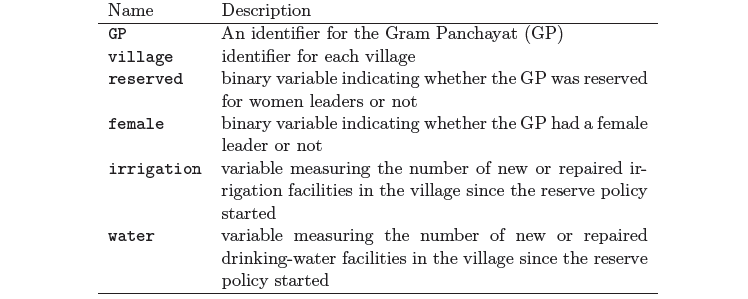
\includegraphics[width=1.1\textwidth]{women_desc.png}
\end{figure}		

\newpage
\begin{enumerate}
	\item [(a)] State a null and alternative (two-tailed) hypothesis. 

\underline{Null hypothesis:} The reservation policy has no effect on the number of new or repaired drinking water facilities in the villages.

\underline{Alternative hypothesis}: The reservation policy has a significant effect (either positive or negative) on the number of new or repaired drinking water facilities in the villages.

	
	\vspace{2cm}
	\item [(b)] Run a bivariate regression to test this hypothesis in \texttt{R} (include your code!).
	
	To test the hypothesis, we can run a bivariate regression with the number of new or repaired drinking water facilities as the dependent variable and the reservation policy as the independent variable. Here's the code:
	
	```{r}
	I$Load the data
	women <- read.csv("https://raw.githubusercontent.com/kosukeimai/qss/master/PREDICTION/women.csv")
	$
	I$Run the regression
	reg <- lm(women$water~women$reservation)
$	
	I$View the results
	summary(reg)
$	
	\vspace{2cm}
	\item [(c)] Interpret the coefficient estimate for reservation policy. 
\end{enumerate}

The coefficient estimate for the reservation policy in the regression represents the expected change in the number of new or repaired drinking water facilities associated with a one-unit increase in the reservation policy (i.e. when a village council head is reserved for women). 

In this case, the coefficient estimate is 0.346, which means that villages with a female council head have, on average, 0.346 more new or repaired drinking water facilities than villages with a male council head. 

Since the p-value for the coefficient estimate is less than 0.05, we can conclude that the effect of the reservation policy on the number of new or repaired drinking water facilities is statistically significant at the 5% level.

\end{document}
